\documentclass{article}
\usepackage[utf8]{inputenc}

\documentclass[a4paper]{article}
\usepackage[14pt]{extsizes} % для того чтобы задать нестандартный 14-ый размер шрифта
\usepackage[utf8]{inputenc}
\usepackage[russian]{babel}
\usepackage{setspace,amsmath}
\usepackage{movie15}
\usepackage{hyperref}

\usepackage{indentfirst}
\usepackage{graphicx}
\usepackage{listings}
\usepackage[left=20mm, top=15mm, right=15mm, bottom=15mm, nohead, footskip=10mm]{geometry} % настройки полей документа
 
\begin{document} % начало документа
 
% НАЧАЛО ТИТУЛЬНОГО ЛИСТА
\begin{center}
\hfill \break
\large{МИНЕСТЕРСТВО НАУКИ И ВЫСШЕГО ОБРАЗОВАНИЯ РОССИЙСКОЙ ФЕДЕРАЦИИ}\\
\footnotesize{ФЕДЕРАЛЬНОЕ ГОСУДАРСТВЕННОЕ БЮДЖЕТНОЕ ОБРАЗОВАТЕЛЬНОЕ УЧРЕЖДЕНИЕ}\\ 
\footnotesize{ВЫСШЕГО ОБРАЗОВАНИЯ}\\
\small{\textbf{«БЕЛГОРОДСКИЙ ГОСУДАРСТВЕННЫЙ ТЕХНОЛОГИЧЕСКИЙ УНИВЕРСИТЕТ ИМ. В.Г. Шухова»}\\
\hfill \break
\hfill \break
\hfill \break
\hfill \break
\hfill\break
\hfill \break
\hfill \break
\hfill \break
\normalsize{Расчётно-графическое задание\\
\large{Разработка web-приложения}\\
\hfill \break
\hfill \break
\hfill \break
\hfill \break
\hfill \break
\end{center}
 
\hfill \break
\hfill \break
 
\normalsize{ 
\begin{center}
\raggedleft{Выполнил: ст. гр. ВТ-191\\Фахретдинов Владислав Станиславович}
\\
\hfill \break
\raggedleft{Проверил: ст.преп.\\Картамышев Сергей Владимирович}
\\
\end{center}
}\\
\hfill \break
\hfill \break
\hfill \break
\hfill \break
\hfill \break
\begin{center} Белгород 2022 \end{center}
\thispagestyle{empty} % выключаем отображение номера для этой страницы
 
\newpage
    \tableofcontents % Вывод содержания
\newpage
 
\newpage

\section{Введение}
На текущий момент, разработка web-приложений является одной из самых распространённых областей в мире, так как охватывает наибольшее количество устройств, а использование этих приложений не требует ничего, кроме браузера. Мы имеем множество платформ, начиная от социальных сетей, стриминг площадок, интернет магазинов и дистрибьюторов, информационных и обучающих ресурсов, которые представляют из себя web-приложения и которыми мы пользуемся каждый день для своего удобства и получения образования и новых навыков, удовольствия, веселья и так далее.

В качестве цели, в данной работе был выбран сайт-визитка - <<Лаборатория анализа данных Владислава Фахретдинова>>, который будет предоставлять информацию о гипотетической "компании".

\section{Проектирование}
Для того, чтобы начинать разработку, нам необходимо представлять себе структуру сайта, его особенности и функционал. 
Так как наш сайт будет представлять из себя визитку компании, мы хотим иметь несколько "страничек", которые будут предоставлять основную информацию.
\begin{enumerate}
    \item Главная страница, на которой будут описаны примерные предоставляемые услуги.
    \item Демонстрация, на которой можно будет воспользоваться одной из современных разработок. \\ 
          В качестве демонстрации, выберем суммаризацию текста, одну из распространённых задач.
    \item Страница отзывов, на которой будет несколько отзывов от наших клиентов.
    \item Страница контактов, на которой будут представлены сотрудники лаборатории, с описанием должностей и возможностей.
\end{enumerate}
Помимо этого, наш сайт будет иметь титульную верхнюю часть страницы, с помощью которой можно будет переключаться между описанными выше страничками.

Для реализации всего этого, будем использовать JavaScript фреймворк Vue, который является одним из самых популярных фреймворков на текущий момент. В его плюсы входит отличная документация со множеством примеров, адаптивность, превосходная интеграция, масштабирование.

Описав примерный интерфейс, теперь нам необходимо понять и описать, что и как наш сайт будет получать от сервера. В нашем случае, для каждой из страничек 1, 3 и 4, описанных выше, потребуется получение лишь одного списка примерно похожих элементов. Для 2 страницы, нам необходимо будет передавать текст, набранный пользователем, на сервер, и получать в ответ суммаризованный текст для дальнейшего его отображения. Запросы к серверу будем делать с помощью библиотеки axios.

В качестве языка программирования и фреймворка, для написание серверной части, были выбраны python и Django из-за их простоты и возможности гибкой реализации и плотной интеграции с другими модулями.
Хранение данных для отображения будем проводить в SQLite, так как объём информации небольшой, не требуется высокая производительность, а сами данные простые и между ними нет сложных связей (услуги, отзывы, контакты).

Наконец, можем перейти к разработке.


\section{Создание frontend стороны на Vue}

 Web-приложение на Vue состоит из двух основных логических блоков - <<View>> или страниц, и <<Component>> или же компонент. 
 
 Страницы из себя представляют какую-то часть реальных страниц на сайте, которые можно переиспользовать вместо других, оставляя при этом некоторые фиксированными. В нашем случе, для каждой из страницы которые мы описывали во введение, будет представлено соответствующее View - ServicesView, DemoView, ReviewsView и ContactsView.
 
 В свою очередь, компоненты представляют ещё меньший кусок страницы, обычно это элементарные единицы, которые зачастую могут быть представлены на страницу в виде нескольких экземпляров, в которых изменяется только информация. Мы будем создавать такие компоненты, как Service, Review, Demo, Contact и  Link, а также Header и Footer, которые будут оставаться на каждой из страниц.
 
 Код страниц, или же View, представляет из себя несколько секций. Первая из секция, это <template>, которая задаёт разметку страницы на адаптированном под нужны Vue HTML, в нёй можно описывать создание компонент, а также использовать классически блоки, которые мы использовали ранее. Также одной из важных секций является <style>, в которой мы описываем наши стили, по аналогии с css, которые будут применяться к нашей разметке. Есть также <script> секция, в которйо мы описываем наше View, его методы, способы получения информации, используемые компоненты, создание данных и обращение к серверу - всю основную часть, которая работает невидимо для обычного пользователя, и позволяет сайту быть таким, каким мы его задумываем.
 
 Код компонент состоит из тех же блоков, но логически представляется оно по другому. Секция <template> теперь описывает один блок с переданной ему информацией, а <style> настраивает как раз взаимодействие не между элементами, как во View, а внутри одного элемента.


\section{Создание backend стороны на Django}
Наш сервер будет отвечать за реализацию API, по которому frontend часть сможет получать информацию. Будем реализовывать четыре метода. Три из них будут GET, то есть отдавать нам информацию на наш запрос, это services, reviews, contacts. И один из них будет POST, он уже будет отдавать нашу информацию в модифицированном виде - это demo. 

Для сохранения данных, в Django сущесвуют модели, которые позволяют воспользоваться ORM подходом.
Опишем наши модели данных: 

\begin{lstlisting}
class Service(models.Model):

    title = models.CharField(max_length=30)
    image = models.ImageField()
    text = models.TextField()

    def __str__(self):
        return self.title


class Review(models.Model):

    text = models.TextField()

    def __str__(self):
        return self.text[:20]


class Contact(models.Model):

    image = models.ImageField()
    fullname = models.CharField(max_length=30)
    title = models.CharField(max_length=30)
    description = models.TextField()

    def __str__(self):
        return self.fullname





class Link(models.Model):
    logo = models.ImageField()
    url = models.CharField(max_length=30)
    contact = models.ForeignKey(Contact, on_delete=models.CASCADE)

    def __str__(self):
        return self.
\end{lstlisting}      

После того, как мы задали модели для наших данных, осталось реализовать методы, которые будут отвечать на запросы и отдавать информацию. Используя модели, по большей части эти методы представляют из себя получение всех объектов и формирование json'a а в том формате, в котором мы принимаем его на frontend стороне. 


\section{Полученные результаты}
После длительного процесса вёртски и создания интерфейса, формирования модели данных, согласования самим с собой api для получения этих данных, реализации отправки их с сервера - можем сказать, что сайт готов. Посмотреть на UI можно по ссылке: \href{https://emperornao.github.io/web/}{https://emperornao.github.io/web/}.

Также, весь код доступен в репозитории \href{https://github.com/EmperorNao/web}{https://github.com/EmperorNao/web}.

\begin{figure}[h!]
    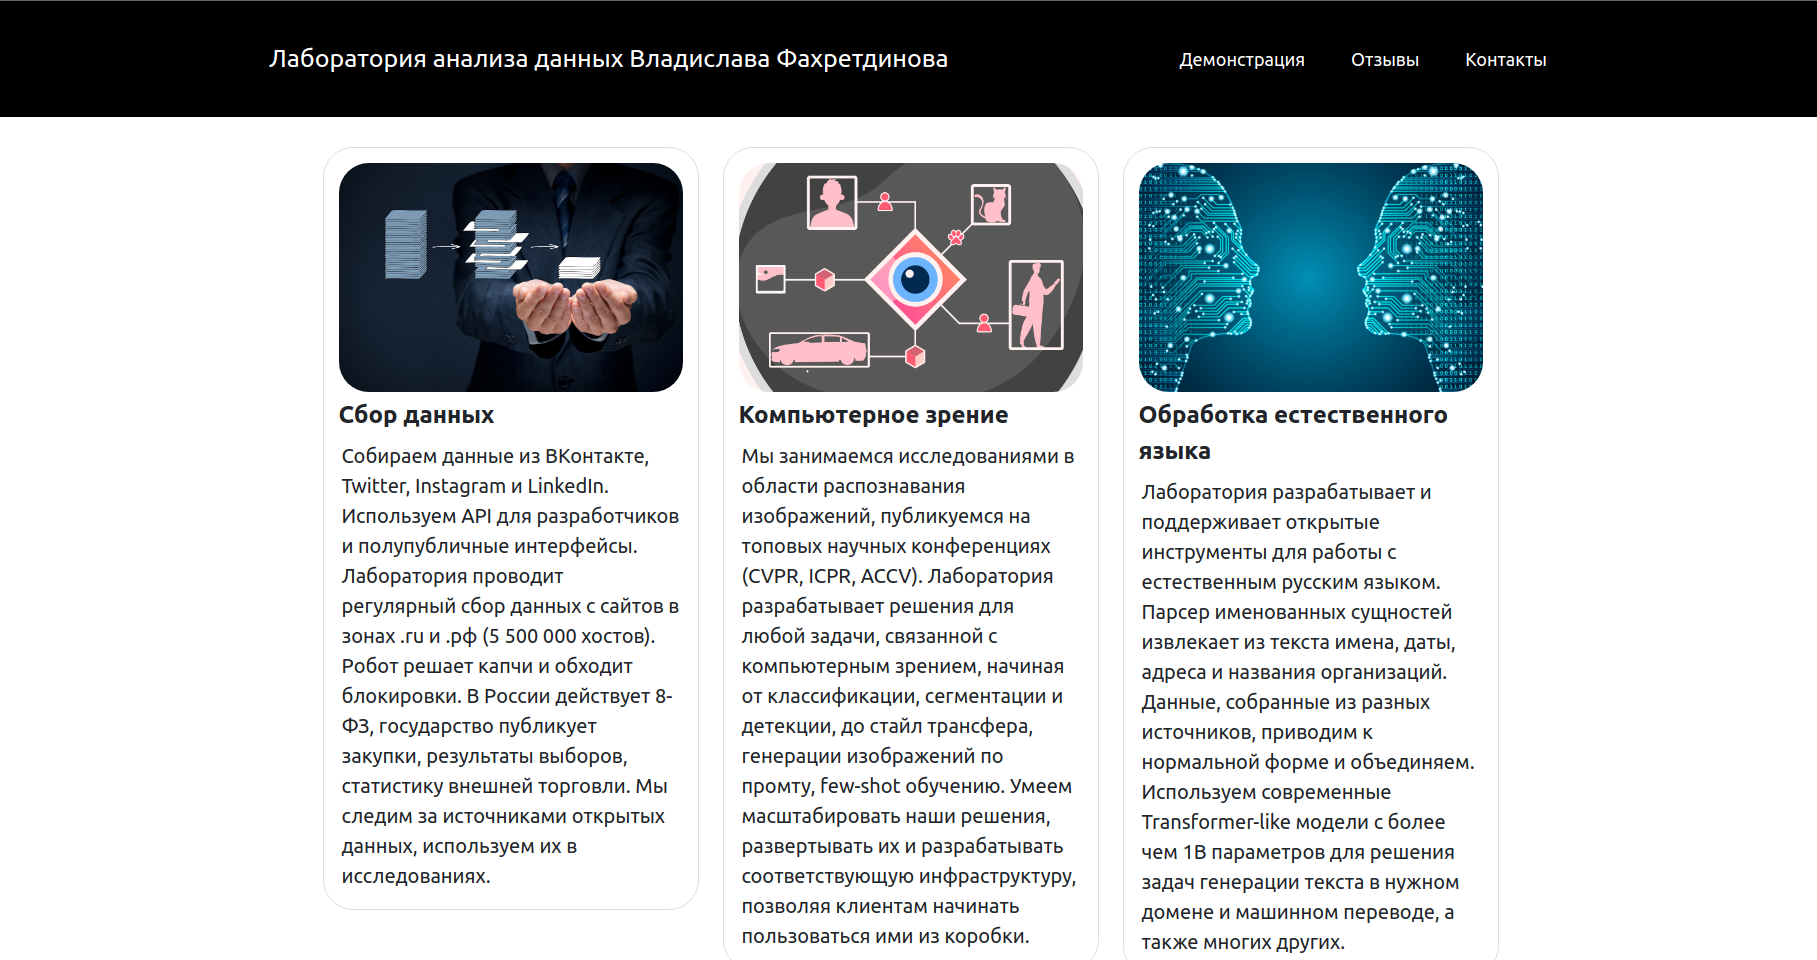
\includegraphics[scale=0.28]{services.png}
    \caption{Главная страница}
\end{figure}

\begin{figure}[h!]
    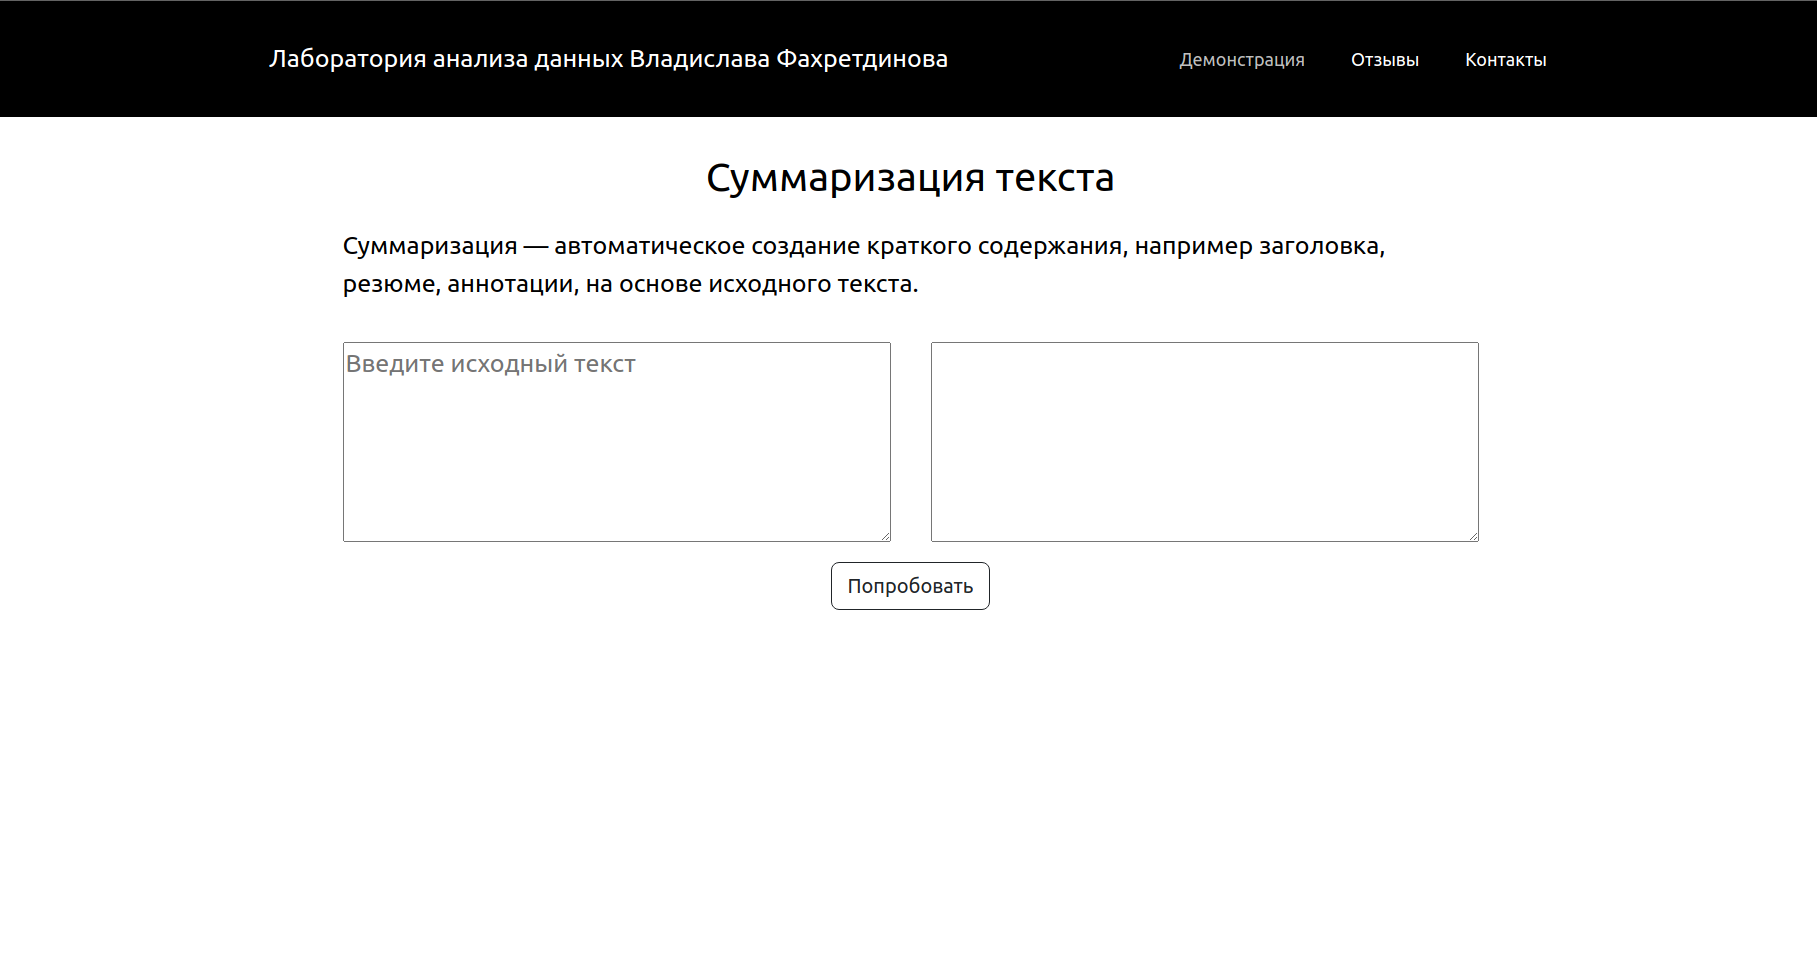
\includegraphics[scale=0.28]{demo.png}
    \caption{Демонстрация}
\end{figure}

\begin{figure}[h!]
    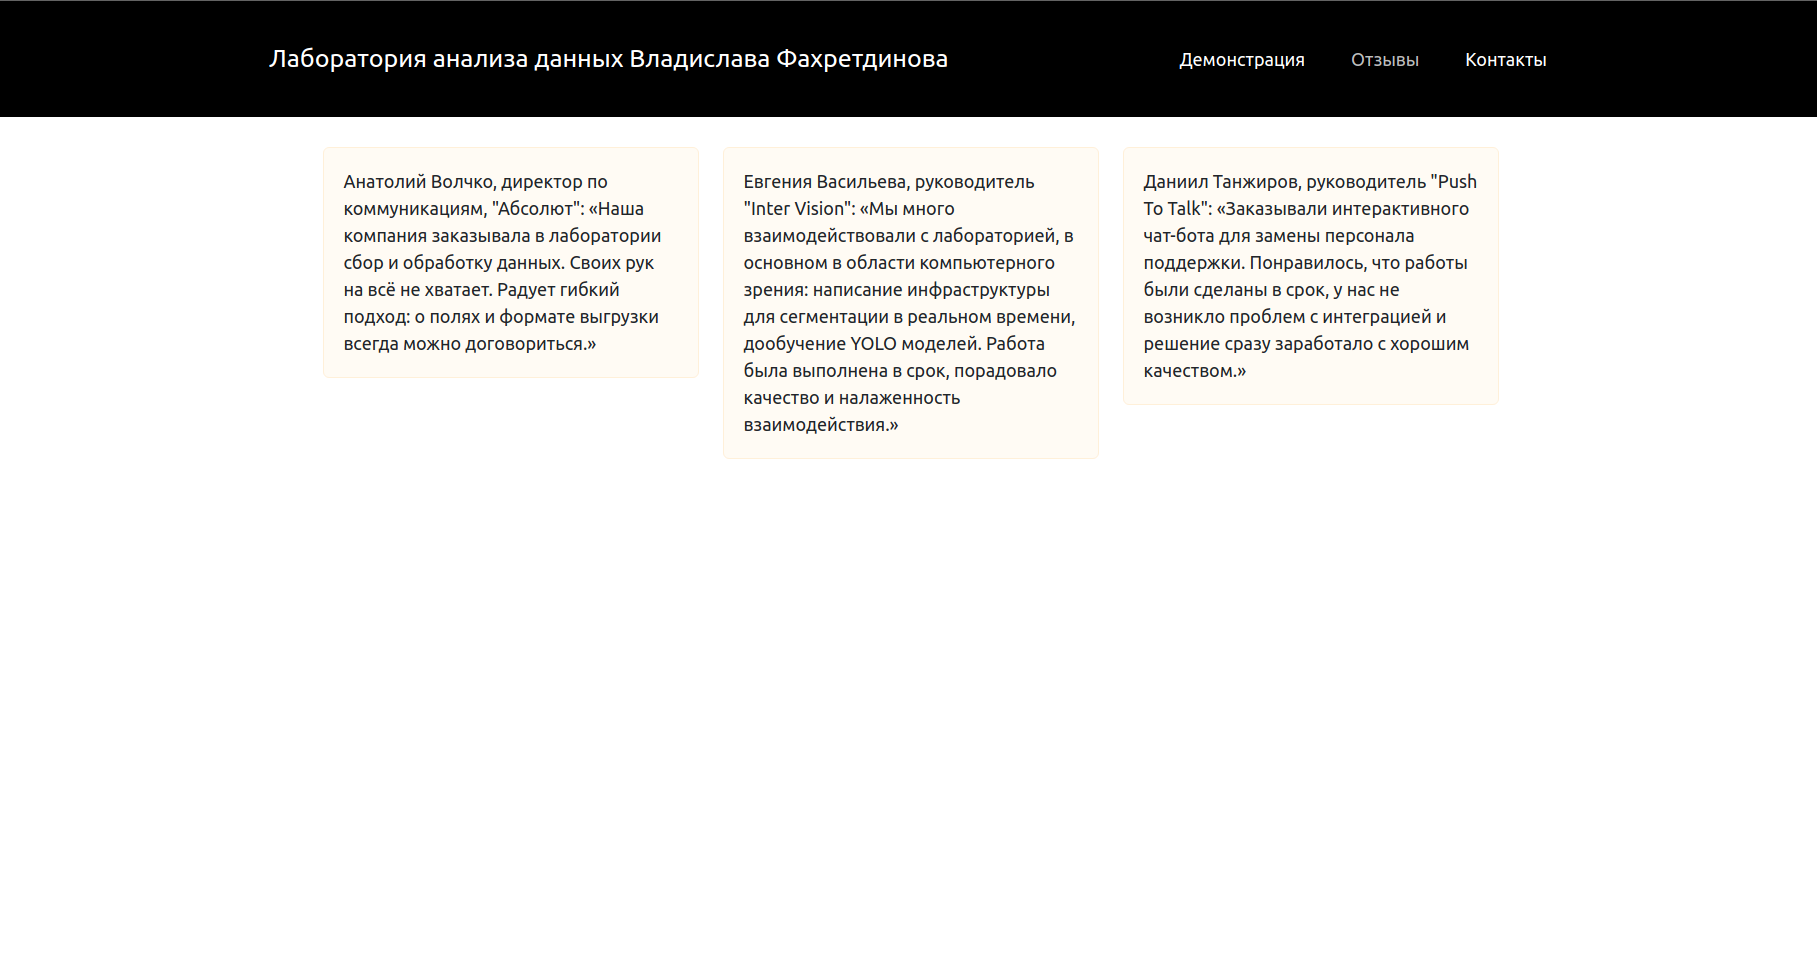
\includegraphics[scale=0.28]{reviews.png}
    \caption{Отзывы}
\end{figure}

\begin{figure}[h!]
    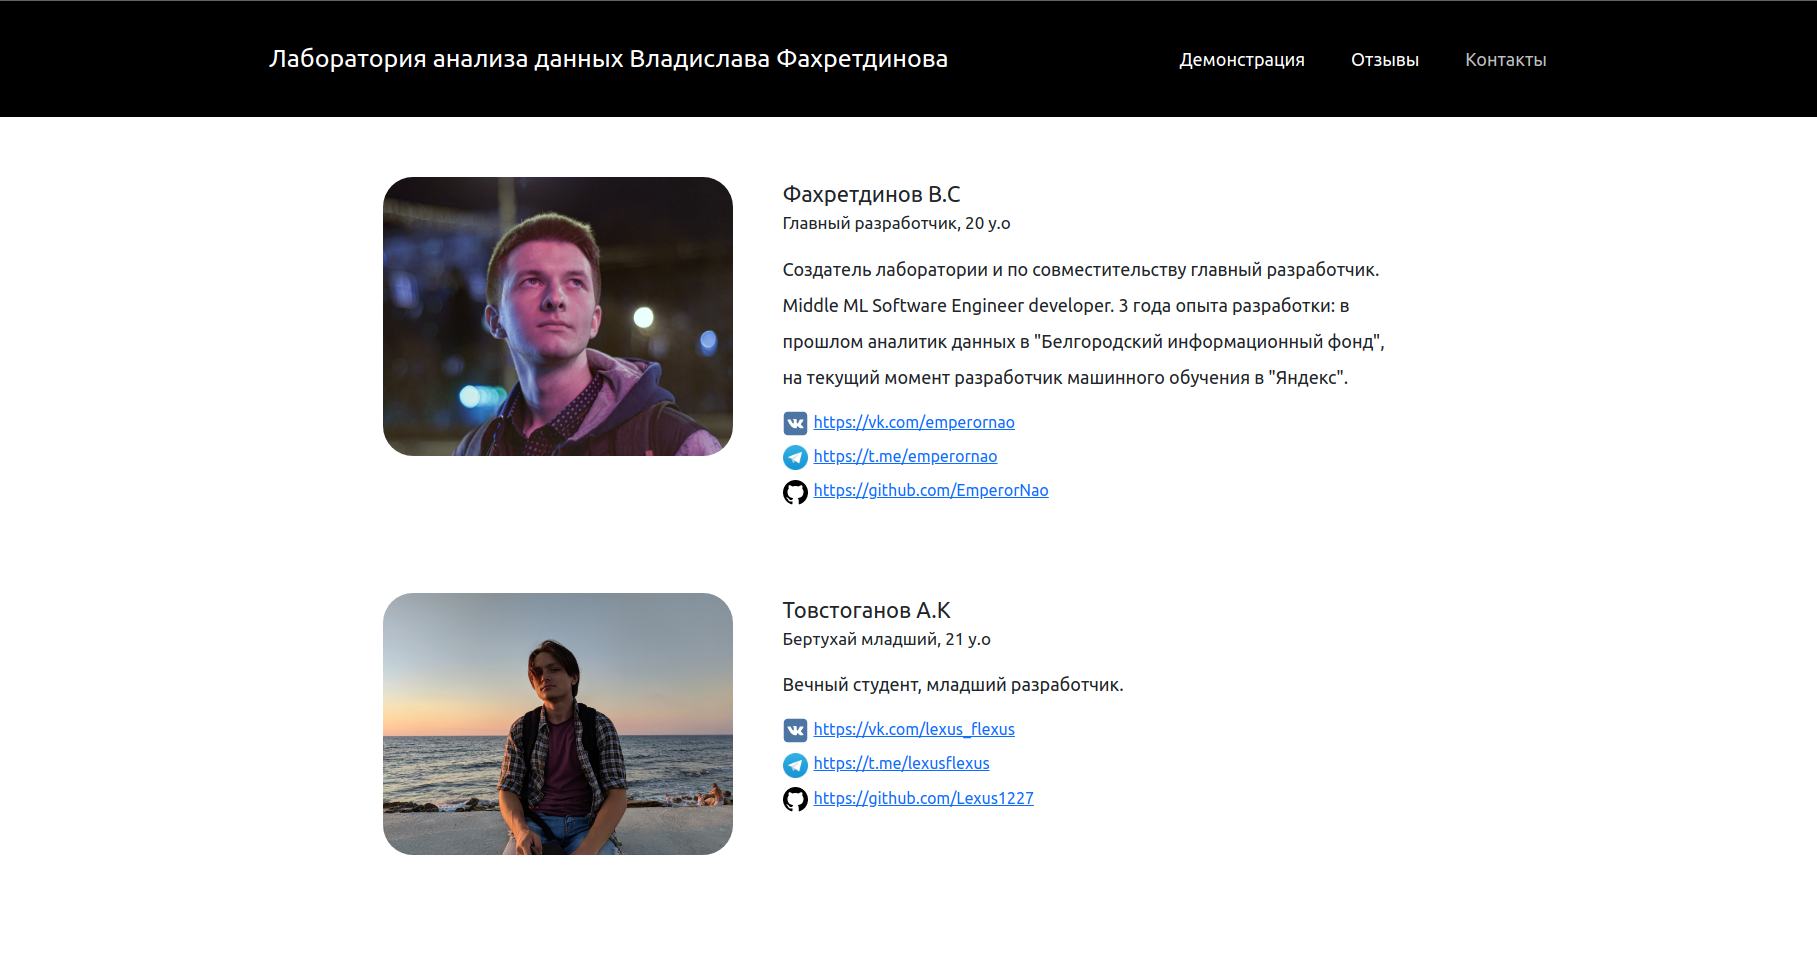
\includegraphics[scale=0.28]{contacts.png}
    \caption{Контакты}
\end{figure}
 
\end{document} 
